\begin{figure}

\centering

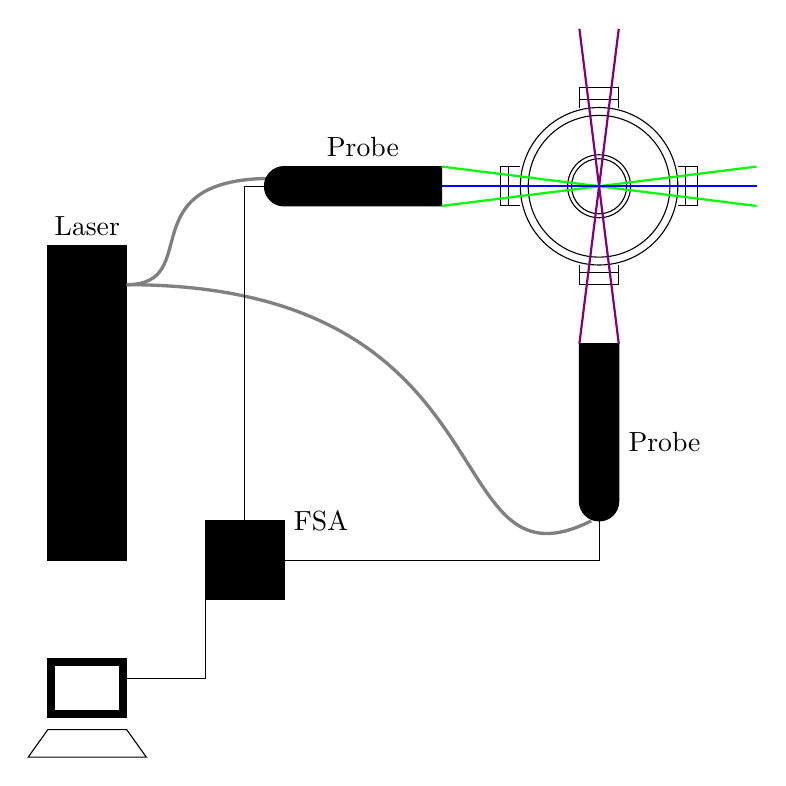
\begin{tikzpicture}

% Pressure vessel, quartz tube
\draw ( 6, 6.75 ) circle ( 1 );
\draw ( 6, 6.75 ) circle ( 0.9 );

\draw ( 5, 6.5 ) -- ++( -0.25, 0 ) -- ++( 0, 0.5 ) -- ++( 0.25, 0 );
\draw ( 5.75, 7.75 ) -- ++( 0, 0.25 ) -- ++( 0.5, 0 ) -- ++( 0, -0.25 );
\draw ( 7, 6.5 ) -- ++( 0.25, 0 ) -- ++( 0, 0.5 ) -- ++( -0.25, 0 );
\draw ( 5.75, 5.75 ) -- ++( 0, -0.25 ) -- ++( 0.5, 0 ) -- ++( 0, 0.25 );

\draw ( 4.85, 6.5 ) -- ++( 0, 0.5 );
\draw ( 5.75, 7.85 ) -- ++( 0.5, 0 );
\draw ( 7.1, 6.5 ) -- ++( 0, 0.5 );
\draw ( 5.75, 5.65 ) -- ++( 0.5, 0 );

\draw ( 6, 6.75 ) circle ( 0.4 );
\draw ( 6, 6.75 ) circle ( 0.35 );

% Laser
\filldraw ( -1, 2 ) rectangle ++( 1, 4 );

% Fiber optic cables
\draw [very thick, gray] ( 0, 5.5 ) .. controls +( 1, 0 ) and +( -1.85, 0 ) .. ++( 1.85, 1.35 );
\draw [very thick, gray] ( 0, 5.5 ) .. controls +( 5, 0 ) and +( -2, -1 ) .. ++( 5.9, -3 );

% Probe A
\filldraw [black] ( 4, 7 ) -- ++( 0, -0.5 ) -- ++( -2, 0 ) arc ( 270:90:0.25 ) -- cycle;

\draw ( 1.75, 6.75 ) -- ++( -0.25, 0 ) -- ++( 0, -4.25 );

% Probe B
\filldraw [black] ( 5.75, 4.75 ) -- ++( 0.5, 0 ) -- ++( 0, -2 ) arc ( 0:-180:0.25 ) -- cycle;

\draw ( 6, 2.5 ) -- ++( 0, -0.5 ) -- ++( -4, 0 );

% Laser beams
\draw[green,thick] ( 4, 7 ) -- ++( 4, -0.5 );
\draw[green,thick] ( 4, 6.5 ) -- ++( 4, 0.5 );
\draw[blue,thick] ( 4, 6.75 ) -- ++( 4, 0 );
\draw[violet,thick] ( 5.75, 4.75 ) -- ++( 0.5, 4 );
\draw[violet,thick] ( 6.25, 4.75 ) -- ++( -0.5, 4 ) ;

% FSA
\filldraw [black] ( 1, 1.5 ) rectangle ++( 1, 1 );

% Computer
\filldraw [black] ( -1, 0 ) rectangle ++( 1, 0.75 );
\filldraw [white]( -0.9, 0.1 ) rectangle ++( 0.8, 0.55 );
\draw ( -1, -0.15 ) -- ++( 1, 0 ) -- ++( 0.25, -0.35 ) -- ++( -1.5, 0 ) -- cycle;

\draw ( 0, 0.5 ) -- ++( 1, 0 ) -- ++( 0, 1 );

% Labels
\node at ( -0.5, 6 ) [above] {Laser};
\node at ( 2, 2.5 ) [right] {FSA};
\node at ( 6.25, 3.5 ) [right] {Probe};
\node at ( 3, 7.25 ) {Probe};

\end{tikzpicture}

\caption[Schematic of the LDV setup]{The schematic shows the setup employed to map the velocity field of the LSB combustor using Laser Doppler Velocimetry. Three pairs of orthogonal beams are separated from the Argon Ion Laser output and conveyed by fiber optic cables (\textcolor{gray}{gray}) to optical probes mounted 90\(^\circ\) apart about the axis of the LSB combustor. The \textcolor{green}{green}, \textcolor{blue}{blue}, and \textcolor{violet}{violet} beams in the schematic represent the 514 nm, 488 nm and 476 nm wavelengths. The signal is collected by the transceiver probes and analyzed by the FSA module. The results are saved for further analysis.}

\label{fig:ldvSetup}

\end{figure}

